\chapter{Detalles de Implementación y Experimentos}\label{chapter:implementation}

En este capítulo se describe detalladamente el proceso de implementación del método propuesto para la mejora de imágenes de tomografía computarizada cerebral. Se presentan las herramientas y entornos de desarrollo empleados, así como las adaptaciones realizadas sobre las implementaciones existentes de la transformada synchrosqueezed (SST) y su inversa (ISST) en el contexto de la transformada curvelet bidimensional (2DCT). Además, se explican los procedimientos seguidos para el preprocesamiento de los datos, la configuración de los experimentos y la aplicación de las distintas estrategias de modificación de la matriz de energía. Finalmente, se justifica la selección de los parámetros experimentales y se expone la estructura general del flujo de trabajo, sentando las bases para la posterior evaluación y comparación de los resultados obtenidos.

\section{Ambiente de trabajo y herramientas}\label{section:work-environment}

El funcionamiento principal de los experimentos gira alrededor de la implementación original de las funciones de SST e ISST, por Haizhao Yang y Lexing Ying \cite{SynchrosqueezedCurveletTransform_SynLab}. Esta fue originalmente concebida en \texttt{Matlab}, un software y lenguaje de programación matemático, con gran énfasis en la practicidad y en la facilidad de uso para personal del sector científico. Esta implementación, con cambios mínimos, fue exportada a \texttt{GNU Octave}, una versión gratuita y de código abierto creada y mantenida por una extensa comunidad de contribuidores. Esto se hizo con el objetivo de poder utilizarlo sin la restricción de las barreras de pago, que en nuestro país se hace de gran dificultad. Esta implementación se encuentra modularizada en el repositorio de la tesis.

Dada la elevada dificultad de la implementación de SST y de ISST, además de la complejidad para crear experimentos complejos y paralelizables para mejor rendimiento, esta fue usada solo como una librería dinámica la cual fue llamada desde \texttt{Python 3.13}. Para esto, se usó la librería \texttt{oct2py}, la cual permite integración directa con el motor de \texttt{Octave} para llamar a las funciones definidas (en este caso solo SST e ISST) con objetos nativos de \texttt{Python}, como son arreglos n-dimensionales de \texttt{numpy}.

Durante el desarrollo y la ejecución de los experimentos, el código fue implementado y ejecutado íntegramente en la unidad central de procesamiento (CPU) de un equipo portátil de alto rendimiento. Este sistema cuenta con un procesador AMD Ryzen 7 8845HS de 8 núcleos y 16 hilos, con una frecuencia base de 3.8 GHz y una frecuencia máxima de hasta 5.1 GHz. Además, dispone de 32 GB de memoria RAM DDR5 y una unidad de almacenamiento sólido (SSD) de 1 TB. Todas las tareas de procesamiento, incluidas las etapas más intensivas computacionalmente, se realizaron exclusivamente en la CPU, sin recurrir a aceleración por hardware gráfico. Estas especificaciones proporcionaron un entorno adecuado para evaluar el rendimiento y la escalabilidad de la implementación propuesta, asegurando resultados reproducibles y tiempos de ejecución competitivos.

Adicionalmente, para el manejo, procesamiento y análisis de los resultados, se emplearon diversas herramientas del ecosistema científico de Python, tales como \texttt{numpy} para operaciones matriciales y de álgebra lineal, \texttt{matplotlib} para la visualización de datos y \texttt{pandas} para la manipulación de conjuntos de datos. El desarrollo de scripts experimentales, automatización de pruebas y gestión de resultados se realizó en un entorno de desarrollo basado en \texttt{Jupyter Notebook}, lo que facilitó la documentación interactiva y la reproducibilidad de los experimentos. Para el control de versiones y la colaboración, se utilizó el sistema \texttt{git}, permitiendo un seguimiento detallado de los cambios y la integración eficiente de mejoras en el código fuente. Finalmente, la ejecución de los experimentos se gestionó mediante scripts de automatización en \texttt{bash} y el uso de entornos virtuales con \texttt{conda} para asegurar la compatibilidad y portabilidad de las dependencias empleadas a lo largo del proyecto.

Para garantizar la reproducibilidad de los resultados y la consistencia en los experimentos, se fijaron explícitamente las semillas aleatorias y las configuraciones relevantes en todos los procesos. Esto permitió obtener resultados comparables y facilitar la validación de los procedimientos implementados.

\section{Optimización de la implementación}\label{section:optimization}

Con el objetivo de mejorar la eficiencia y el rendimiento de la solución propuesta, se han incorporado las siguientes optimizaciones en la implementación:

\begin{itemize}
    \item \textbf{Caché de los datos obtenidos:} Se ha implementado un sistema de almacenamiento temporal de los datos intermedios, como son el resultado de aplicar SST sobre una imagen en particular. Esta estrategia permite reutilizar resultados previamente calculados y reducir el acceso a la memoria principal o la necesidad de recomputar información, lo que se traduce en una disminución significativa del tiempo de ejecución global.
    
    \item \textbf{Paralelización de la ejecución:} Se ha aprovechado la capacidad de procesamiento concurrente de \texttt{Python} mediante la paralelización del procesamiento de imágenes independientes. Esto permite distribuir la carga de trabajo entre múltiples núcleos o hilos, acelerando etapas críticas como el cálculo de transformadas y la reconstrucción de imágenes, y logrando una mejora sustancial en los tiempos de cómputo.
    
    \item \textbf{Limpieza de los objetos no utilizados en memoria:} Para evitar la acumulación innecesaria de datos y prevenir posibles fugas de memoria, se ha incorporado un mecanismo de liberación sistemática de los objetos que ya no son requeridos durante la ejecución. Esta gestión eficiente de la memoria contribuye a mantener la estabilidad y el rendimiento de la aplicación, especialmente en experimentos de gran escala o en entornos con recursos limitados.
\end{itemize}

La necesidad de implementar optimizaciones en el procesamiento de imágenes surge de las exigencias computacionales observadas durante el desarrollo experimental. En primer lugar, el resultado de la SST aplicada a una sola imagen puede ocupar aproximadamente 1.4 GB de espacio en memoria, lo que representa una carga significativa para los recursos del sistema. Además, los tiempos de ejecución para el procesamiento completo de una imagen —incluyendo tanto la SST como su inversa (ISST)— alcanzan una media de 4 minutos, lo que limita la viabilidad del método en escenarios donde se requiere el análisis de grandes volúmenes de datos o la respuesta en tiempo real. Por otro lado, el consumo de memoria RAM sin la aplicación de optimizaciones puede llegar a ser muy intenso, alcanzando picos de hasta 15 GB durante la ejecución de múltiples experimentos. Estas condiciones motivan la incorporación de técnicas específicas de optimización, orientadas a reducir el uso de memoria, agilizar los tiempos de procesamiento y garantizar la estabilidad del sistema, permitiendo así la aplicación práctica y eficiente del método propuesto en entornos computacionales con recursos limitados.

Como resultado de las optimizaciones implementadas, se logró una reducción significativa tanto en los tiempos de ejecución como en el consumo de memoria del sistema. Tras la aplicación de estas mejoras, el tiempo medio de procesamiento por experimento —incluyendo la aplicación de SST e ISST sobre una imagen— disminuyó a aproximadamente 2 minutos, lo que representa una mejora sustancial en la eficiencia operativa del método. Asimismo, el uso máximo de memoria RAM durante la ejecución se redujo a 4 GB, permitiendo la realización de experimentos en equipos con recursos más limitados y mejorando la estabilidad general del sistema durante la ejecución de múltiples tareas en paralelo. Estos resultados evidencian la efectividad de las estrategias de optimización adoptadas en el desarrollo de la presente implementación.

\section{Implementación de los experimentos} \label{section:experiment-implementation}

La implementación de los experimentos se basa en un flujo modular que permite el procesamiento eficiente y reproducible de imágenes. El proceso inicia con la carga y normalización de las imágenes, que pueden provenir tanto de archivos individuales en formatos estándar (\texttt{.jpg} o \texttt{png}) como de volúmenes médicos (\texttt{.nii}). Para la gestión y muestreo de imágenes, se emplean objetos utilitarios que permiten recuperar conjuntos de imágenes desde directorios estructurados, facilitando la selección aleatoria o secuencial de muestras para los experimentos.

En cuanto al preprocesamiento, este se aplicó de manera diferenciada según la naturaleza de los experimentos. En una primera serie de experimentos, las imágenes fueron normalizadas para que sus valores de intensidad se encontraran en el rango $[0, 1]$. Esta normalización permitió asegurar la homogeneidad en la escala de entrada y facilitó la comparación directa entre diferentes muestras, independientemente de su origen o condiciones de adquisición.

En una segunda serie de experimentos, se utilizaron imágenes volumétricas en formato \texttt{.nii}, sobre las cuales se aplicó una ventana de intensidad específica para procesar únicamente la sección correspondiente a la densidad del cerebro. Esta técnica de ventana permitió resaltar las estructuras anatómicas de interés y reducir el impacto de regiones irrelevantes o valores atípicos, optimizando así la calidad y relevancia de los datos utilizados en el análisis posterior.

Cabe destacar que la naturaleza del preprocesamiento aplicado influyó notablemente en los tiempos de ejecución de los experimentos. En la primera serie, al trabajar con imágenes normalizadas en un rango reducido de valores, los tiempos de procesamiento fueron considerablemente menores, con una media aproximada de 1 minuto por experimento. En contraste, la segunda serie, basada en imágenes volumétricas procesadas mediante la aplicación de una ventana de intensidad, presentó tiempos de ejecución significativamente mayores, oscilando entre 3 y 5 minutos por experimento. Esta diferencia en el rendimiento también tuvo implicaciones directas en los resultados obtenidos, las cuales serán analizadas en detalle en una sección posterior.% todo

Una vez cargadas y preprocesadas, las imágenes son transformadas mediante la aplicación de la transformada synchrosqueezed curvelet y su inversa. Este procedimiento se encuentra encapsulado en objetos que gestionan tanto la ejecución de las transformadas como la utilización de un sistema de caché, el cual almacena los resultados intermedios para evitar recomputaciones innecesarias y optimizar el uso de recursos. Los resultados de la transformada se almacenan en estructuras especializadas que contienen la energía synchrosqueezed, los coeficientes curvelet y los vectores asociados, permitiendo su manipulación eficiente en las siguientes etapas del experimento.

Las funciones experimentales, están implementadas como procedimientos puros que operan sobre los resultados de la transformada, generando nuevas instancias modificadas de dichos resultados sin alterar los datos originales. La ejecución de cada experimento se gestiona a través de utilidades que reciben una configuración detallada, especificando la función experimental a aplicar, los parámetros y los argumentos adicionales requeridos. Tras la aplicación de la función experimental, se realiza la reconstrucción de la imagen modificada mediante la transformada inversa, asegurando la consistencia del flujo de procesamiento.

Durante todo el proceso, se implementa un sistema de registro para el seguimiento detallado de cada etapa y la gestión de errores. Además, se asegura la reproducibilidad de los experimentos mediante la fijación de semillas aleatorias y la serialización de los resultados y configuraciones empleadas. Este enfoque modular y estructurado permite realizar experimentos complejos de manera eficiente, garantizando la trazabilidad y la robustez de los resultados obtenidos.

El flujo completo de procesamiento experimental se organiza a través de una función principal que recibe como entrada un conjunto de imágenes, las configuraciones específicas de los experimentos a realizar y las configuraciones de las métricas de evaluación. Internamente, esta función itera sobre cada imagen y, para cada una, aplica de manera secuencial las distintas configuraciones experimentales definidas. Para cada combinación de imagen y configuración experimental, se ejecuta el procesamiento correspondiente: primero se realiza la transformada synchrosqueezed sobre la imagen, luego se aplica la función experimental seleccionada sobre los resultados de la transformada, y finalmente se reconstruye la imagen modificada mediante la transformada inversa.

Durante este proceso, se calculan las métricas de evaluación especificadas, comparando la imagen reconstruida con la original u otras referencias según corresponda. Todos los resultados, así como los parámetros y configuraciones utilizados, se almacenan y registran de forma estructurada para su posterior análisis. Este proceso automatizado permite ejecutar grandes volúmenes de experimentos de manera eficiente, garantizando la trazabilidad y la reproducibilidad (ver imagen \ref{fig:diagrama-flujo-experimentos}).

\begin{figure}[H]
    \centering
    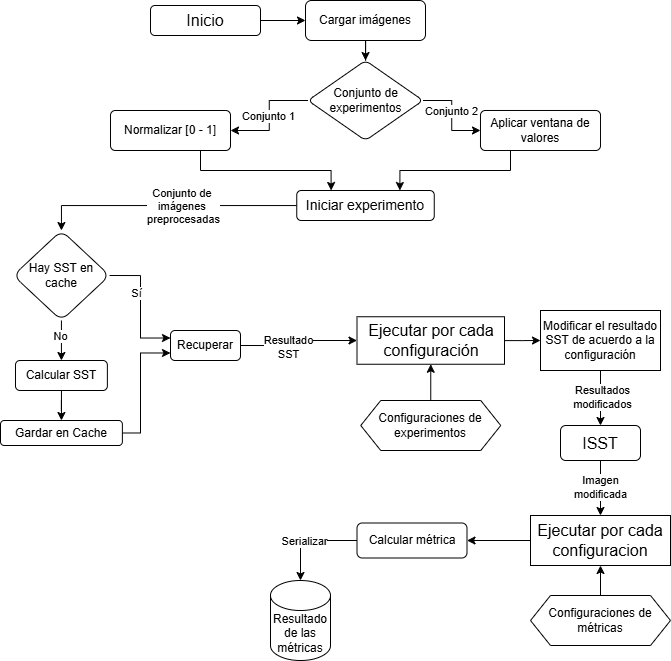
\includegraphics[width=0.95\textwidth]{Graphics/diagrama experimentos tesis.drawio.png}
    \caption{Diagrama de flujo del pipeline experimental implementado para el procesamiento y análisis de imágenes. El diagrama ilustra las etapas principales: carga y preprocesamiento de imágenes, aplicación de la transformada synchrosqueezed curvelet, ejecución de funciones experimentales, reconstrucción, cálculo de métricas y almacenamiento estructurado de resultados.}
    \label{fig:diagrama-flujo-experimentos}
\end{figure}

\begin{table}[h]
    \centering
    \caption{Configuraciones experimentales y sus parámetros.\cite{ExperimentSource,ExperimentSource2}}
    \label{tab:experimentos}
    \begin{tabular}{>{\raggedright}p{4cm}p{6cm}}
    \toprule
    \textbf{Tipo de Experimento} & \textbf{Parámetros} \\ 
    \midrule
    Umbralizado & threshold = 0.1, 0.05, 0.001 \\
    \midrule
    Mejora de energía & \texttt{enhancement\_factor} = 3.0, 1.5, 10 \\
    \midrule
    Filtro pasa-alto & \texttt{cutoff\_scale} = 5, 10 \\
    \midrule
    Filtro pasa-banda & \texttt{low\_scale} = 5 (\texttt{high\_scale} = 10), 15 (20) \\
    \midrule
    Máscara gaussiana & $ \mu  = N/2$, $ \sigma $ = 1.0, 4.0, 6.0 \\
    \midrule
    Máscara exponencial & \texttt{decay\_rate} = 0.1, 0.01 \\
    \bottomrule
    \end{tabular}
    \footnotesize{\\*N/2: mitad de las escalas disponibles en la descomposición.}
\end{table}

Para la realización de los experimentos se utilizó un conjunto de configuraciones específicas, las cuales se detallan en la Tabla~\ref{tab:experimentos}. Cada configuración define los parámetros y valores empleados en las distintas funciones experimentales aplicadas durante el procesamiento, permitiendo así evaluar el comportamiento del método bajo diferentes condiciones y ajustes. Esta variedad de configuraciones facilita un análisis exhaustivo y comparativo de los resultados obtenidos.

\section{Implementación de las métricas} \label{section:metrics-implementation}

Las métricas utilizadas para la evaluación cuantitativa de los resultados experimentales fueron implementadas de manera modular y eficiente, empleando herramientas especializadas del ecosistema científico de \texttt{Python}. Las configuraciones específicas de las métricas se encuentran detalladas en la Tabla~\ref{tab:metricas}

Para las métricas basadas en operaciones numéricas y estadísticas, como el índice de mejora de contraste y la razón de nitidez basada en el operador Laplaciano, se utilizó la biblioteca \texttt{numpy} para el cálculo vectorizado de desviaciones estándar y varianzas, así como \texttt{opencv-python} para la aplicación de operadores de filtrado espacial.

Las métricas perceptuales avanzadas, como el FSIM (Feature Similarity Index) y LPIPS (Learned Perceptual Image Patch Similarity), se implementaron a través de las bibliotecas \texttt{piq} y \texttt{lpips}, respectivamente, haciendo uso de \texttt{PyTorch} para el manejo de tensores y la ejecución eficiente en CPU. El índice de similitud estructural (SSIM) y la relación señal-ruido pico (PSNR) se calcularon utilizando las funciones \texttt{structural\_similarity} y \texttt{peak\_signal\_noise\_ratio} de la biblioteca \texttt{scikit-image}. Para la métrica BRISQUE, orientada a la evaluación de artefactos y ruido perceptual, se empleó la implementación disponible en \texttt{piq}.

El flujo de cálculo de métricas se integra al final de cada experimento: una vez reconstruida la imagen modificada, se aplican de forma automática todas las métricas relevantes, comparando la imagen procesada con la original o con una referencia apropiada (en este caso, con la imagen original). Cada función de métrica está desacoplada del resto del procesamiento y recibe como entrada los arreglos de imagen en formato \texttt{numpy}, asegurando así su reutilización y extensibilidad.

Los resultados de cada métrica, junto con la configuración experimental correspondiente, son almacenados y registrados de forma estructurada al finalizar cada experimento. Este enfoque garantiza la trazabilidad y facilita el análisis comparativo entre diferentes configuraciones y tipos de preprocesamiento. Además, la modularidad de la implementación permite la fácil incorporación de nuevas métricas en futuras extensiones del trabajo.

De manera concreta, para cada imagen procesada, una vez ejecutados todos los experimentos definidos, se calculan de forma automática todas las métricas seleccionadas para cada resultado. Posteriormente, los valores obtenidos de las métricas, junto con la información sobre la imagen y la configuración experimental utilizada, son serializados y almacenados en un archivo en formato \texttt{json}. Esta estrategia permite centralizar y organizar los datos de evaluación, facilitando su análisis posterior, la comparación sistemática entre diferentes métodos y la integración con herramientas externas de análisis estadístico o visualización.

\begin{table}[h]
    \centering
    \caption{Métricas de evaluación agrupadas por categorías\cite{Metrics}}
    \label{tab:metricas}
    \begin{tabular}{p{3cm}p{8cm}p{3cm}}
    \toprule
    \textbf{Categoría} & \textbf{Métrica} & \textbf{Descripción} \\ 
    \midrule
    \multirow{3}{*}{Mejora} 
    & CII (\textit{Contrast Improvement Index}) & Índice de mejora de contraste \\
    & LSR (\textit{Laplacian Sharpness Ratio}) & Cociente de nitidez Laplaciana \\
    & FSIM (\textit{Feature Similarity Index}) & Similaridad de características \\
    \midrule

    \multirow{3}{*}{Distorsión}
    & PSNR (\textit{Peak Signal-to-Noise Ratio}) & Relación señal-ruido \\
    & SSIM (\textit{Structural Similarity Index}) & Similaridad estructural \\
    & LPIPS (\textit{Learned Perceptual Image Patch Similarity}) & Similaridad perceptual \\
    \midrule

    \multirow{2}{*}{Artefactos}
    & RNS (Residual Noise Standard Deviation) & Desviación estándar del ruido residual \\
    & BRISQUE (Blind/Referenceless Image Spatial Quality Evaluator \cite{BRISQUE}) & Evaluador ciego de calidad \\
    \bottomrule
    \end{tabular}
\end{table}

\section{Implementación de las estadísticas}\label{section:statistics-implementation}

El análisis estadístico de los resultados experimentales se diseñó para comparar de manera rigurosa el desempeño de los distintos métodos evaluados. Para cada par de experimentos a comparar, se recopilaron los valores obtenidos de las métricas correspondientes en todas las imágenes procesadas. El primer paso consistió en la aplicación de pruebas de normalidad sobre la distribución de cada métrica, con el objetivo de determinar el tipo de análisis estadístico adecuado para la comparación. Las pruebas de normalidad empleadas incluyeron, entre otras, la prueba de Shapiro-Wilk.

En función de los resultados de la prueba de normalidad, se seleccionó el método estadístico más apropiado para la comparación de los dos grupos experimentales. Cuando la distribución de las métricas fue compatible con la normalidad, se utilizó la prueba t de Student para muestras independientes, permitiendo evaluar si existían diferencias estadísticamente significativas entre las medias de los grupos. En caso contrario, es decir, si la distribución no era normal, se recurrió a pruebas no paramétricas como la prueba de Mann-Whitney U, que permite comparar la mediana de dos muestras independientes sin asumir normalidad.

Si el análisis estadístico indicó que existían diferencias significativas entre los experimentos comparados, se procedió a comparar sus medias y desviaciones estándar para cada métrica, determinando así cuál de los dos experimentos presentaba un mejor desempeño según los valores observados. En caso de que no se detectaran diferencias estadísticamente significativas, se asumió que ambos experimentos ofrecían resultados equivalentes para la métrica analizada.

\begin{table}[h]
    \centering
    \caption{Resumen de las métricas utilizadas, sus valores ideales y rangos de referencia.}
    \label{tab:metrics-expected-values}
    \begin{tabular}{>{\raggedright}p{5cm}p{3cm}p{3cm}}
        \toprule
        \textbf{Métrica} & \textbf{Valor ideal} & \textbf{Rango} \\
        \midrule
        Índice de mejora de contraste (CII) & $>1$ & $[0, \infty)$ \\
        Razón laplaciana & $>1$ & $[0, \infty)$ \\
        FSIM & $1$ & $[0, 1]$ \\
        PSNR & $\infty$ & $[0, \infty)$ \\
        SSIM & $1$ & $[0, 1]$ \\
        LPIPS & $0$ & $[0, 1]$ \\
        Desviación estándar del ruido residual & $0$ & $[0, \infty)$ \\
        BRISQUE & $0$ & $[0, 100]$ \\
        \bottomrule
    \end{tabular}
\end{table}

Adicionalmente, para cada métrica se consultó una tabla de valores esperados o ideales (Tabla~\ref{tab:metrics-expected-values}), lo que permitió contextualizar los resultados obtenidos y seleccionar el experimento más favorable dentro de cada par comparado. En este proceso, se otorgó un peso mayor a aquellas métricas consideradas prioritarias para la calidad de la imagen, como el índice de similitud estructural (SSIM), que evalúa la preservación de la estructura, y la métrica de nitidez basada en el operador Laplaciano, que prioriza la definición de bordes. Esta ponderación permitió orientar la selección final hacia los experimentos que maximizan la fidelidad estructural y la nitidez en las imágenes reconstruidas.

Para el análisis estadístico de los resultados experimentales se emplearon principalmente las bibliotecas \texttt{pandas} para la manipulación y análisis de los datos tabulados, y \texttt{scipy.stats} para la ejecución de pruebas estadísticas como el test de normalidad y las pruebas de comparación entre grupos. Adicionalmente, las bibliotecas \texttt{seaborn} y \texttt{matplotlib.pyplot} se utilizaron para la visualización gráfica de los resultados y la exploración de tendencias y distribuciones. Estas herramientas permitieron realizar un análisis estadístico riguroso, reproducible y visualmente comprensible de los datos obtenidos en los experimentos.
